\documentclass[12pt, letterpaper]{scrartcl}

\usepackage{fullpage} % Set margins and place page numbers at bottom center
\usepackage[shortlabels]{enumitem} % Use a. in the enumerate
\usepackage{amsmath} % aligned equations
\usepackage{graphicx} % include figure
\usepackage{float} % usage of H for figure float
\usepackage{amssymb} % \blacksqure and \triangleq
\usepackage{xcolor} % color in math mode

\begin{document}

% ### Header - start ###
    \begin{center}
    	\hrule
    	\vspace{0.4cm}
    	{\textbf { {\large Homework 2} \\ EE 668 --- Information Theory}}
    \end{center}
    { \textbf{Name:} Ali Zafari \hspace{\fill} \textbf{Student Number:} 800350381 \hspace{\fill} \textbf{Fall 2022} } \newline\hrule
% ### Header - end ###

\paragraph*{Problem 2.1} \hfill\newline
\begin{enumerate}[((a))]
    \item According to \textbf{central limit theorem}, $M_n$ will follow a normal distribution with mean and variance of the data distribution divided by the sample sequence size, i.e., $Exp(1)$:
    \begin{align*}
        M_n&\sim \mathcal{N}(E[X], \frac{Var[X]}{n})\\
        M_n&\sim \mathcal{N}(1, \frac{1}{n})\\
    \end{align*}
    We can define $A_n$ being defined as $A_n\triangleq\frac{M_n-1}{1/\sqrt{n}}$:
    \begin{align*}
        A_n&\sim \mathcal{N}(0, 1)\\
    \end{align*}
    Hence, the probability can be written in terms of Q-function of a Standard Normal($\Phi$):
    \begin{align*}
        P[M_n>2]&=P[A_n>\sqrt{n}]\\
        &=\Phi(\sqrt{n})
    \end{align*}
    \begin{figure}[H]
        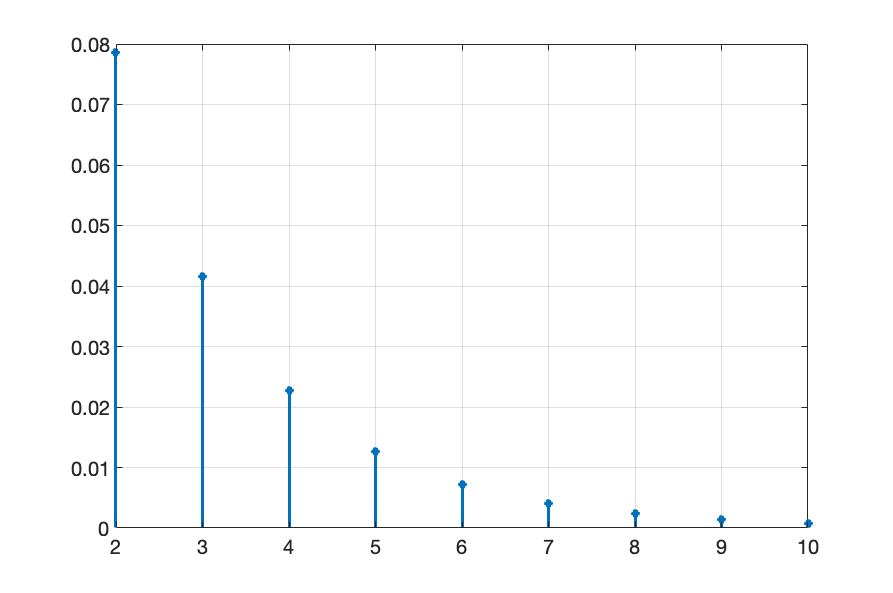
\includegraphics[width=0.6\linewidth]{hw2_figures/2.1a.png}
        \centering
        \caption{$P(M_n>2)$}
    \end{figure}
    \item To develop the Chernoff bound on the probability distribution of the sample mean, we recall (from EE 513):
    \begin{align*}
        P[M_n>\gamma]\leq e^{-\max\limits_{s\geq 0}\{s\gamma-\phi_{M_n}(s)\}}
    \end{align*}
    where $\phi_{M_n}(s)$ is the logarithm of the moment generating function (log-MGF).\\\\
    As $M_n\sim \mathcal{N}(1, \frac{1}{n})$, its MGF function would be:
    \begin{align*}
        \textrm{(MGF)}\qquad\Phi_{M_n}(s)&=e^{\mu s+\frac{\sigma_{M_n}^2}{2}s^2}\\
        &=e^{s+\frac{s^2}{2n}}\\
        \textrm{(log-MGF)}\quad\Rightarrow\phi_{M_n}(s)&=s+\frac{s^2}{2n}
    \end{align*}
    To find the value of $s$ which maximized the exponent, we set its derivative equal to zero:
    \begin{align*}
        \frac{d}{ds}(s(\gamma-1)-\frac{s^2}{2n})\bigg\rvert_{s^*}=\gamma-1-\frac{s}{n}\bigg\rvert_{s^*}=0\Rightarrow s^*=n
    \end{align*}
    Finally the Chernoff bound will be as follows, by having $\gamma=2$:
    \begin{align*}
        P[M_n>2]&\leq e^{-\{n\times2-n-\frac{n}{2}\}}\\
        P[M_n>2]&\leq e^{-\frac{n}{2}}\\
    \end{align*}
    \begin{figure}[H]
        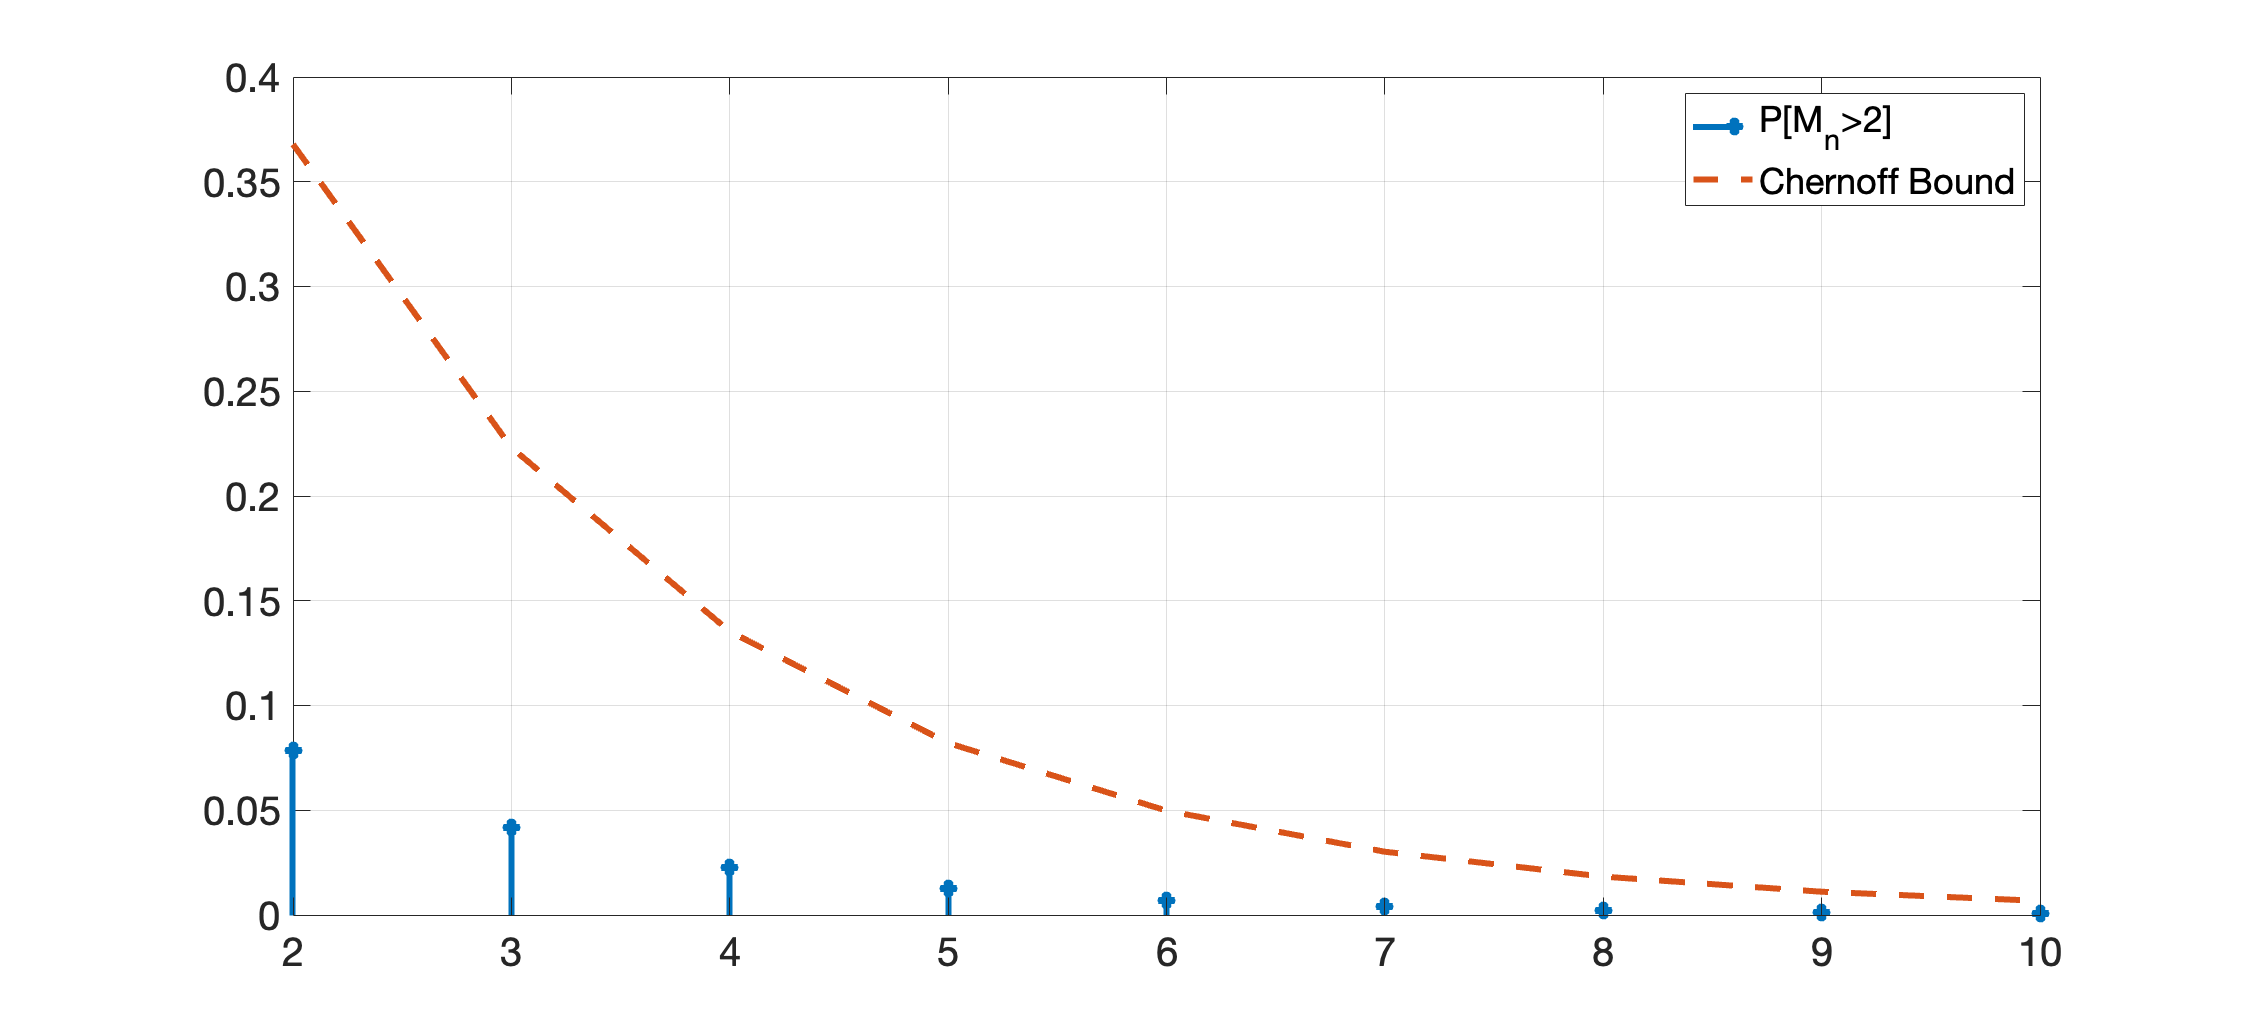
\includegraphics[width=0.8\linewidth]{hw2_figures/2.1b.png}
        \centering
        \caption{Chernoff Bound vs. $P(M_n>2)$}
    \end{figure}
\end{enumerate}
\hrule
\paragraph*{Problem 2.2} \hfill\newline
\begin{enumerate}[((a))]
    \item Let's define $A_n$ as the product of the drawn samples:
    \begin{align*}
        A_n=(X_1X_2\dots X_n)^\frac{1}{n}
    \end{align*}
    then 
    \begin{align*}
        \log A_n=\frac{1}{n}\log(X_1X_2\dots X_n)=\frac{1}{n}\sum_{i=1}^n\log X_i
    \end{align*}
    Now we can infer that $\log A_n$ is the sample mean of the random variable $Y$ being defined as $Y\triangleq\log X$.\\\\
    By using the strong law of large numbers:
    \begin{align*}
        \begin{matrix}{}\\{\overline {Y}}_{n}\ {\xrightarrow {Prob.=1}}\ \mu_Y \qquad {\textrm {when}}\ n\to +\infty\\{}\end{matrix}
    \end{align*}
    so we only need to calculate $\mu_Y$:
    \begin{align*}
        \mu_Y&=E_{y\sim f_Y(y)}[Y]\\
        &=E_{x\sim f_X(x)}[\log X]\\
        &=\frac{1}{2}\log1+\frac{1}{4}\log2+\frac{1}{4}\log3\\
        &=\frac{1}{4}\log 6
    \end{align*}
    Therefore:
    \begin{align*}
        \begin{matrix}{}{\overline {Y}}_{n}=\log A_n\ {\xrightarrow {Prob.=1}}\ \log6^{\frac{1}{4}} \qquad {\textrm {when}}\ n\to +\infty{}\end{matrix}
    \end{align*}
    \begin{align*}
        \begin{matrix}{}{{A}}_{n}=(X_1X_2\dots X_n)^\frac{1}{n}\ {\xrightarrow {Prob.=1}}\ 1.5650 \qquad {\textrm {when}}\ n\to +\infty{}\end{matrix}
    \end{align*}
    
    \item Entropy of $X$:
    \begin{align*}
        H(X)&=-\sum p\log p\\
        &=-(\frac{1}{2}\log\frac{1}{2}+\frac{1}{4}\log\frac{1}{4}+\frac{1}{4}\log\frac{1}{4})\\
        &=1.5
    \end{align*}
\end{enumerate}
\hrule
\paragraph*{Problem 2.3} \hfill\newline
\begin{enumerate}[((a))]
    \item
    \begin{align*}
        \lim_{n\rightarrow+\infty}\left[-\frac{1}{n}\log q(X_1,X_2,\dots,X_n)\right]=\lim_{n\rightarrow+\infty}\left[-\frac{1}{n}\sum_{i=1}^n\log q(X_i)\right]
    \end{align*}
    Now we can infer that the above limit is on the sample mean of the random variable $Y$ being defined as $Y\triangleq-\log q(X_i)$.\\\\
    By using the strong law of large numbers:
    \begin{align*}
        \begin{matrix}{}\\{\overline {Y}}_{n}\ {\xrightarrow {Prob.=1}}\ \mu_Y \qquad {\textrm {when}}\ n\to +\infty\\{}\end{matrix}
    \end{align*}
    so we only need to calculate $\mu_Y$:
    \begin{align*}
        \mu_Y&=E_{y\sim f_Y(y)}[y]\\
        &=E_{x\sim f_X(x)}[-\log q(x_i)]\\
        &=-\sum_{i=1}^{n}p(x_i)\log q(x_i)\\
        &=-\sum_{i=1}^{n}p(x_i)\log[q(x_i)\times\mathbin{\color{blue}\frac{p(x_i)}{p(x_i)}}]\\
        &=\sum_{i=1}^{n}p(x_i)\log\frac{p(x_i)}{q(x_i)}-\sum_{i=1}^{n}p(x_i)\log p(x_i)\\
        &=D(p||q)+H(p)
    \end{align*}
    
    \item 
    \begin{align*}
        \lim_{n\rightarrow+\infty}\left[\frac{1}{n}\log\frac{q(X_1,X_2,\dots,X_n)}{p(X_1,X_2,\dots,X_n)}\right]=\lim_{n\rightarrow+\infty}\left[\frac{1}{n}\sum_{i=1}^n\log\frac{q(X_i)}{p(X_i)}\right]
    \end{align*}
    Now we can infer that the above limit is on the sample mean of the random variable $Y$ being defined as $Y\triangleq\log\frac{q(X)}{p(X)}$.\\\\
    By using the strong law of large numbers:
    \begin{align*}
        \begin{matrix}{}\\{\overline {Y}}_{n}\ {\xrightarrow {Prob.=1}}\ \mu_Y \qquad {\textrm {when}}\ n\to +\infty\\{}\end{matrix}
    \end{align*}
    so we only need to calculate $\mu_Y$:
    \begin{align*}
        \mu_Y&=E_{y\sim f_Y(y)}[y]\\
        &=E_{x\sim f_X(x)}[\log\frac{q(x)}{p(x)}]\\
        &=\sum_{i=1}^{n}p(x_i)\log\frac{q(x_i)}{p(x_i)}\\
        &=-D(p||q)
    \end{align*}
\end{enumerate}
\hrule
\paragraph*{Problem 2.4} \hfill\newline
\begin{align*}
    \log l=\frac{1}{n}\ln V_n=\frac{1}{n}\sum_{i=1}^{n}\ln X_i
\end{align*}
Now we can infer that $\ln l$ is the sample mean of the random variable $Y$ being defined as $Y\triangleq\ln X$.\\\\
By using the strong law of large numbers:
\begin{align*}
    \begin{matrix}{}\\{\overline {Y}}_{n}\ {\xrightarrow {Prob.=1}}\ \mu_Y \qquad {\textrm {when}}\ n\to +\infty\\{}\end{matrix}
\end{align*}
so we only need to calculate $\mu_Y$:
\begin{align*}
    \mu_Y&=E_{y\sim f_Y(y)}[Y]\\
    &=E_{x\sim f_X(x)}[\ln X]\\
    &=\int_0^1\ln xdx\\
    &=x(\ln x-1)\bigg\rvert_0^1\\
    &=-1
\end{align*}
Hence:
\begin{align*}
    \begin{matrix}{}{\overline {Y}}_{n}=\ln l\ {\xrightarrow {Prob.=1}}\ -1 \qquad {\textrm {when}}\ n\to +\infty{}\end{matrix}
\end{align*}
\begin{align*}
    \begin{matrix}{}\\{l}\ {\xrightarrow {Prob.=1}}\ e^{-1}=0.3679 \qquad {\textrm {when}}\ n\to +\infty\\{}\end{matrix}
\end{align*}
\hrule
\end{document}

